% Shared preamble for the three ENS003 software-team presentations.
% Each presentation \input{}'s this file.

\documentclass[11pt,aspectratio=169]{beamer}

\usepackage[utf8]{inputenc}
\usepackage[T1]{fontenc}
\usepackage{lmodern}
\usepackage{amsmath}
\usepackage{booktabs}
\usepackage{graphicx}
\usepackage{listings}
\usepackage{xcolor}
\usepackage{hyperref}

% Built-in Beamer theme so the deck compiles on any TeX Live / MacTeX
% install without external packages. Customise colours below.
\usetheme{Boadilla}
\usecolortheme{seahorse}
\setbeamertemplate{navigation symbols}{}
\setbeamertemplate{footline}[frame number]

\definecolor{ink}{HTML}{1A1A1A}
\definecolor{accentred}{HTML}{A02828}
\definecolor{accentgreen}{HTML}{2C662C}
\definecolor{codebg}{HTML}{F7F5EE}
\definecolor{rulegrey}{HTML}{888888}

\setbeamercolor{normal text}{fg=ink}
\setbeamercolor{frametitle}{bg=ink, fg=white}
\setbeamercolor{title}{fg=ink}
\setbeamercolor{author}{fg=ink}
\setbeamercolor{date}{fg=rulegrey}
\setbeamercolor{block title}{bg=ink, fg=white}
\setbeamercolor{block body}{bg=codebg, fg=ink}
\setbeamercolor{alerted text}{fg=accentred}
\setbeamercolor{structure}{fg=ink}
\setbeamerfont{frametitle}{series=\bfseries}

\lstset{
  basicstyle=\ttfamily\scriptsize,
  backgroundcolor=\color{codebg},
  language=Python,
  keywordstyle=\color{accentred},
  stringstyle=\color{accentgreen},
  commentstyle=\color{rulegrey}\itshape,
  breaklines=true,
  numbers=none,
  showstringspaces=false,
  frame=single,
  framerule=0pt,
  framesep=6pt,
  xleftmargin=0pt,
  xrightmargin=0pt
}

% Convenience commands
\newcommand{\code}[1]{\texttt{\small #1}}
\newcommand{\file}[1]{\textcolor{accentred}{\texttt{\small #1}}}
\newcommand{\unit}[1]{\,\mathrm{#1}}

% Title-slide metadata is set per-deck (so the same preamble can power
% both Turkish and English versions of each talk).


\newcommand{\courseHeader}{ENS003 --- Digital Twins for Health Sciences}
\newcommand{\courseSubheader}{Istinye University · Faculty of Engineering and Natural Sciences}
\newcommand{\instructor}{Instructor: Prof. Dr. Şenol Pişkin}
\newcommand{\projectTitle}{A Surrogate ML Model for a Ti-6Al-4V Cementless Hip Implant}

\title{Flask Dashboard, Predict CLI and Integration}
\subtitle{\projectTitle}
\author{Ali Edip Mangtay \\ \small Software Engineering · 210911044}
\date{May 2026 \\ \scriptsize \courseHeader{} · \instructor}

\begin{document}

\maketitle

% ---------------------------------------------------------------------------
\begin{frame}{In this talk}
  \begin{itemize}
    \item How I exposed the surrogate to an end user
    \item Architecture choices (Flask + Jinja + Plotly + KaTeX)
    \item The LaTeX-paper aesthetic and why we went that way
    \item Sidebar UX: three continuous sliders + three preset buttons
    \item Two production-flavoured bugs (HTTP 500, cache)
  \end{itemize}
  \vspace{0.4cm}
  \begin{block}{My responsibility (software team)}
    The web app, the predict CLI, templates/static, integration,
    \file{run.sh}.
  \end{block}
\end{frame}

% ---------------------------------------------------------------------------
\begin{frame}{Architecture}
  \begin{columns}[T,onlytextwidth]
    \column{0.5\textwidth}
    \textbf{Server (Python):}
    \begin{itemize}\small
      \item Flask + Jinja2 (HTML rendering)
      \item joblib model loading (10 models at init)
      \item Plotly figure JSON generation
      \item \code{/} (HTML) and \code{/predict} (JSON) endpoints
    \end{itemize}
    \column{0.5\textwidth}
    \textbf{Client (browser):}
    \begin{itemize}\small
      \item Plotly.js (CDN, chart rendering)
      \item KaTeX (CDN, equations)
      \item Vanilla JS slider events
      \item \code{fetch('/predict?...')} for AJAX
    \end{itemize}
  \end{columns}

  \vspace{0.5cm}
  \textbf{Design call:} no bundler, no framework, two libraries via CDN.
  Reason: for an academic deliverable we want \alert{minimum dependencies}
  --- the demo should run on the jury's laptop in seconds.
\end{frame}

% ---------------------------------------------------------------------------
\begin{frame}{The LaTeX-paper aesthetic}
  The dashboard was designed to look like an academic article:
  \begin{itemize}\small
    \item Centered \code{title-block}, authors, instructor, date
    \item An italic-grey \emph{Abstract} section
    \item Numbered sections (1. Loading conditions, 2. Predicted quantities, \ldots)
    \item Inline and display equations rendered with KaTeX
    \item Booktabs-style tables (1.6pt top/bottom rules, thin mid rule)
    \item STIX Two Text serif family (academic PDF feel)
  \end{itemize}

  \vspace{0.4cm}
  \begin{block}{Why bother?}
    \footnotesize
    For the jury demo, we did not want a plain ``ML form'' --- we wanted an
    \alert{interactive extension of the project report}. Our UX lines have
    to match the Beamer/LaTeX aesthetic.
  \end{block}
\end{frame}

% ---------------------------------------------------------------------------
\begin{frame}{Sidebar UX}
  \begin{columns}[T,onlytextwidth]
    \column{0.55\textwidth}
    \textbf{Three continuous sliders:}
    \begin{itemize}\small
      \item \code{mass} --- 40--110 kg
      \item \code{K} --- 2.0--6.0 (body-weight multiplier)
      \item \code{angle} --- 0°--20° (force tilt)
    \end{itemize}
    \vspace{0.3cm}
    \textbf{Three quick-jump preset buttons:}
    \begin{itemize}\small
      \item Walking \(\Rightarrow K = 2.5\)
      \item Stair climbing \(\Rightarrow K = 3.5\)
      \item Running / jumping \(\Rightarrow K = 4.5\)
    \end{itemize}
    \column{0.45\textwidth}
    \textbf{Three SF gauges:}
    \begin{itemize}\small
      \item Neck
      \item STEM 1
      \item STEM 2
    \end{itemize}
    \vspace{0.3cm}
    \textbf{Status callout:}
    driven by \(\min(\text{neck}, \text{stem1}, \text{stem2})\) ---
    labelled Safe / Caution / Critical.
  \end{columns}

  \vspace{0.4cm}
  \footnotesize
  Preset buttons only set the \(K\) slider; mass and angle are left
  alone. Activity is not a categorical input here --- \(K\) is a
  continuous parameter, so a dropdown would impose a fake discreteness.
\end{frame}

% ---------------------------------------------------------------------------
\begin{frame}[fragile]{The predict endpoint}
\begin{lstlisting}
@app.route("/predict")
def predict_endpoint():
    try:
        mass  = float(request.args.get("mass", 70.0))
        K     = float(request.args.get("k", 2.5))
        angle = float(request.args.get("angle", 0.0))
    except (TypeError, ValueError):
        return jsonify(error="invalid query parameters"), 400
    return jsonify(build_payload(mass, K, angle, models, train_df))
\end{lstlisting}

  \vspace{0.3cm}
  \code{build\_payload} runs all 10 models and returns:
  \begin{itemize}\small
    \item \code{input}: \((m, K, \theta, F_x, F_z, |F|)\)
    \item \code{metrics}: 3 SFs + 3 stresses + deformation, all \(\pm\sigma\)
    \item \code{status}: Safe / Caution / Critical
    \item \code{near}: closest FEA row (normalised \((m, K, \theta)\) distance)
    \item \code{figures}: 6 Plotly figure JSON objects
  \end{itemize}
\end{frame}

% ---------------------------------------------------------------------------
\begin{frame}{Bug story: ``The angle slider does nothing''}
  \textbf{Report:} the dashboard \alert{freezes} when θ moves 0→20.

  \vspace{0.4cm}
  \textbf{Failure chain:}
  \begin{enumerate}\small
    \item User picks θ=5 (grid is \{0, 10, 20\}, off-grid)
    \item In \code{comparison\_chart}, the filter
          \code{np.isclose(angle, 5)} returns \alert{zero rows}
    \item Empty pandas Series gets handed to Plotly as an ndarray
    \item Flask \code{jsonify} \(\Rightarrow\) \alert{500: ndarray not JSON serializable}
    \item Frontend \code{if (!resp.ok) return;} \(\Rightarrow\) \alert{silent fail}
    \item The user sees stale values \(\Rightarrow\) ``nothing changed''
  \end{enumerate}

  \vspace{0.3cm}
  \textbf{Fix:} \code{\_nearest\_value()} snaps \((K, \theta)\) to the
  closest grid point, the legend label adapts, and \code{.tolist()} casts
  guard the serializer.
\end{frame}

% ---------------------------------------------------------------------------
\begin{frame}[fragile]{Snap to nearest slice}
\begin{lstlisting}
def _nearest_value(value, options):
    return float(options[int(np.argmin(np.abs(options - value)))])

def comparison_chart(rows, ..., K, angle, ...):
    K_grid = np.sort(rows["K_factor"].unique())
    angle_grid = np.sort(rows["force_angle_deg"].unique())
    K_near = _nearest_value(K, K_grid)
    angle_near = _nearest_value(angle, angle_grid)

    same = rows[
        np.isclose(rows["K_factor"], K_near)
        & np.isclose(rows["force_angle_deg"], angle_near)
    ].sort_values("patient_mass_kg")
    # ... add Scatter trace with .tolist() casts
\end{lstlisting}

  \vspace{0.2cm}
  The legend label adapts automatically:
  \begin{itemize}\small
    \item Exact grid point: ``FEA training (K=2.5, θ=0°)''
    \item Off-grid: ``FEA training (nearest slice K=2.5, θ=0°)''
  \end{itemize}
\end{frame}

% ---------------------------------------------------------------------------
\begin{frame}{Dashboard screenshot}
  \begin{center}
    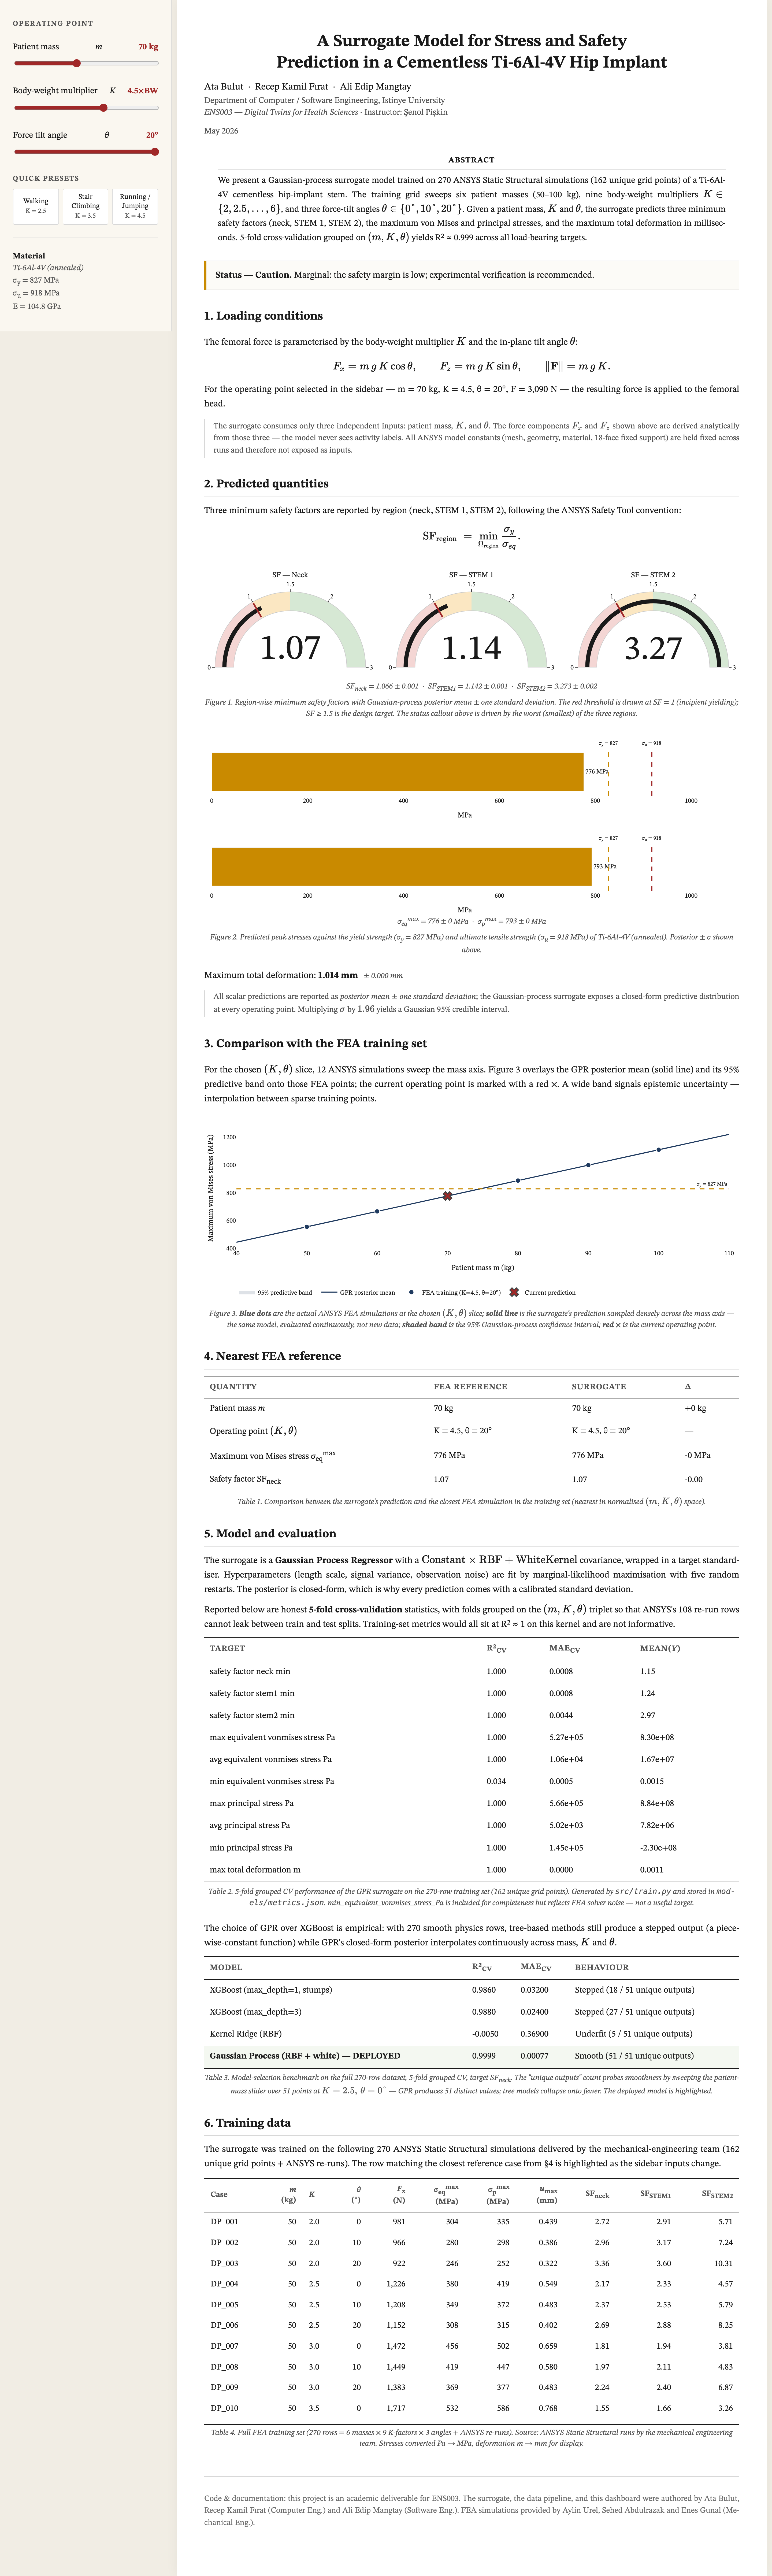
\includegraphics[width=0.78\textwidth]{../../screenshots/desktop_1440__tilted_70kg_K4.5_20deg.png}
  \end{center}
  \vspace{-0.4cm}
  \footnotesize
  Operating point: \(m{=}70\unit{kg}\), \(K{=}4.5\), \(\theta{=}20°\).
  The three SF gauges report SF\(_{\text{neck}}{=}1.07\) (Caution),
  SF\(_{\text{stem2}}{=}3.27\) (Safe). The nearest-FEA panel on the right
  matches an exact training row.
\end{frame}

% ---------------------------------------------------------------------------
\begin{frame}{Polish details}
  \begin{itemize}
    \item \textbf{Cache disabled:} \code{SEND\_FILE\_MAX\_AGE\_DEFAULT=0}
          \(\Rightarrow\) every CSS/JS edit shows up on a normal refresh
          (dev productivity).
    \item \textbf{Mobile sidebar:} \code{@media (max-width: 760px)} gives a
          slide-in panel; hamburger toggle handles open/close.
    \item \textbf{Posterior \(\pm\sigma\) annotations:} GPR's standard
          deviation appears in italic grey next to every gauge and stress bar.
    \item \textbf{Activity preset buttons:} they only set the \(K\) slider
          --- mass and angle stay where the user left them.
    \item \textbf{Training table scroll + sticky thead:} 270 rows, 460px
          height, headers stay pinned while scrolling.
  \end{itemize}
\end{frame}

% ---------------------------------------------------------------------------
\begin{frame}[fragile]{CLI + integration}
\begin{lstlisting}[language=bash, basicstyle=\ttfamily\small]
$ ./run.sh predict --mass 70 --k 2.5 --angle 0
{
  "safety_factor_neck_min": 1.553,
  "safety_factor_stem1_min": 1.662,
  "safety_factor_stem2_min": 5.711,
  "max_equivalent_vonmises_stress_Pa": 532000000.0,
  ...
}

$ ./run.sh predict --mass 80 --activity stair_climbing
# Snaps K to the preset, then predicts.
\end{lstlisting}

  \vspace{0.4cm}
  Both the dashboard and the CLI call the same \code{predict()} function.
  \code{preprocess.add\_features()} is the \alert{single source of truth}.
\end{frame}

% ---------------------------------------------------------------------------
\begin{frame}{Deployment paths (open decision)}
  \textbf{Today:} \code{flask run} dev server, Python deps \(\sim 234\) MB.

  \vspace{0.3cm}
  \textbf{Vercel/Netlify serverless:} 250 MB unzipped limit ---
  right at the edge, with 3--5 s cold starts.

  \vspace{0.4cm}
  \textbf{Candidate routes:}
  \begin{enumerate}\small
    \item Hugging Face Spaces / Render / Railway (Flask as-is)
    \item Push Plotly client-side (saves \(\sim 40\) MB)
    \item \alert{Static precompute:} sample \((m, K, \theta)\) once,
          ship \(\sim 1\) MB gzipped JSON, do trilinear interpolation in
          the browser \(\Rightarrow\) GitHub Pages, zero backend.
    \item Port the GPR to JS (\(\sim\) 100 lines), exact predictions, no server.
  \end{enumerate}

  \vspace{0.3cm}
  The team will pick a path after this talk.
\end{frame}

% ---------------------------------------------------------------------------
\begin{frame}{Questions}
  \vfill
  \begin{center}
    \Large Thank you.\\[0.4cm]
    \normalsize Questions?
  \end{center}
  \vfill
  \scriptsize
  \begin{itemize}
    \item \file{src/app.py}, \file{src/predict.py}, \file{src/templates/}, \file{src/static/}
    \item \file{run.sh} (CLI wrapper)
    \item \file{scripts/capture\_screenshots.py} (dashboard renders)
    \item Sprint log: \file{docs/PROJECT\_NOTES.md} Sprint 4, 7
  \end{itemize}
\end{frame}

\end{document}
